\documentclass[../manuscript]{subfiles}
\def\biblio{\bibliographystyle{plainnat}\bibliography{bibliography}}
\usepackage{Sweave}
\begin{document}

\section[Experiment 2]{Experiment 2. Occlusion.}
\label{sec:occlusion}


%This loads a large data file, which takes a bit of time.
%For better turnaround times, I use cacheSweave

% this explores the statement below that there is not a
% consistent variation between target number and eccentricity
% from the constant stimulus experiment

The results of \nameref{sec:constant} suggest that the perceived direction of incongruent motion stimuli follows the global translation when stimuli are widely spaced, but follows the local motion direction when stimuli are packed more closely together. The between-element spacing at which the percept changes from global-dominated to local-dominated appears to be roughly proportional to the stimulus eccentricity. As a result the stimulus at PSE has approximately the same number of elements, independent of eccentricity. This leaves open an alternate explanation: observers' correct perception of global motion may be limited by the number of simultaneously visible elements rather than their closeness. Such might be the case if subjects were determined the direction by individuating and tracking distinct elements in the display. Humans appear to have a limited capacity for individuating and tracking multiple targets within a scene \citep{Pylyshyn:1988fk}, which might be overwhelmed by displays with large numbers of targets.

The data from \nameref{sec:constant} do not distinguish target number from spacing; there is not a consistent trend for the number of targets at PSE to change as a function of eccentricity. If target tracking capacity may be different for different portions of the visual field, as for example it appears to differ between the lower and upper visual field \citep{He:1996rt}, then \nameref{sec:constant} cannot even in principle differentiate an explanation based on target number from one based on density. To distinguish the effect of target number from that of density, we repeated the measurement of critical spacing with and without an occluder that obscured most of the targets, reducing their number without changing their spacing.

\subsection{Methods}

\todo[inline]{In retrospect, seeing where this analysis is taking me, a much better approach would be to (1) not bother testing at different eccentricities and (2) test varying sizes of the (visible) window!}


Trial structure and timing were as in \nameref{sec:constant}, but with the addition of an occluder that was present or absent on either side of the screen. The occluder was a `C' shape with an opening subtending $120^\circ$ on either the left or right of the screen and covering all eccentricities that a target might appear at. The stimuli are shown schematically in the legend of \autoref{fig:occlusionPSE}, but for the data reported here, the occluder was not visible (i.e. it had the same luminance as the background.)

We decided to test stimuli in the left and right hemifields over separate sessions. If subjects used attentional resources to individuate and track the motion elements, then their spatial allocation of attention may impact performance. Mixing left-visible and right-visible stimuli in the same trial blocks would require subjects to alternately allocate attention to left and right sides, perhaps unnecessarily limiting their performance; preliminary data suggested that a fully interleaved design inflated the critical spacing measurement for occluded conditions \todo{(and this inflation was partially recovered by using a visible occluder that cued the side that targets were to appear on. -- supplementary figure?)} Therefore we measured critical spacing for right and left hemifields in separate sessions. In each session, half of trials contained an occluder and half did not. Note that spatial allocation of attention may also impact subjects' performance in the case that individuation of elements turns out not to be necessary to perform their task.

Instead of the method of constant stimuli we used the QUEST procedure \citep{Watson:1983hc} to select the target density for each trial. A separate QUEST sequence was used to seek the PSE at each eccentricity and for both fully visible and occluded stimuli (so 8 interleaved QUEST sequences for each session) with trials from all sequences being randomly interleaved. As before, there were three trial types, with local motion congruent with global motion, incongruent with global motion, or in counterphase. The online QUEST estimates was used to select target spacing for all trials, but only incongruent trials with responses given during the response window were used to update the online estimates.

In modeling subjects' responses we employed a generalized linear regression using binomial errors and a modified logistic link function with variable upper and lower asymptotes, corresponding to a guess rate and a lapse rate \citep{Wichmann:2001kx}; \todo{I have not actually done this yet; currently it's just a fixed 5\% guess rate.} these rates were allowed to vary between subjects and were iteratively fit to maximize likelihood. Comparisons between nested models were done by likelihood ratio test using a $\chi^2$ distribution with the appropriate number of degrees of freedom depending on the models, as well as by comparisons of Akiake's information criterion (AIC) between models. Before comparing models, guess and lapse rates were first fit to maximize the joint likelihood of both models. For statistics such as the PSE that are not linear functions of the regression coefficients, standard errors and comparisons were computed by parametric bootstrap. \todo{ref?}

\subsection{Results}

\begin{figure}
	\begin{subfigure}[b]{.45\linewidth}
		\includegraphics[width=\linewidth]{a_daily}
		\subcaption{PSE values, measured as in \autoref{fig:constant}. Colors indicate visibility condition (left-visible, right-visible, fully-visible). Shape of data points indicates sessions data were taken on; each measurement in a partially occluded condition is matched with a fully-visible condition taken during the same session.}\label{fig:occlusionPSE}
	\end{subfigure}
	\begin{subfigure}[b]{.45\linewidth}
		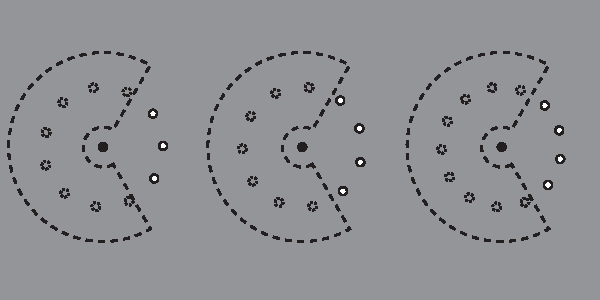
\includegraphics[width=\linewidth]{countDensity}	
		\subcaption{Adding an occluder helps to disentangle target number from target density. Left: out of 11 targets spaced evenly around a circle surrounding the fixation point, two are visible in the non-occluded window. Middle: With a different starting position, four targets are visible with the same target density. Right: Again four targets are visible, but at a higher density (13 targets in the full circle). Thus target density and the number of visible targets are not strictly dependent on each other.}\label{fig:occlusionDensity}
	\end{subfigure}
	\begin{subfigure}[b]{.45\linewidth}
	        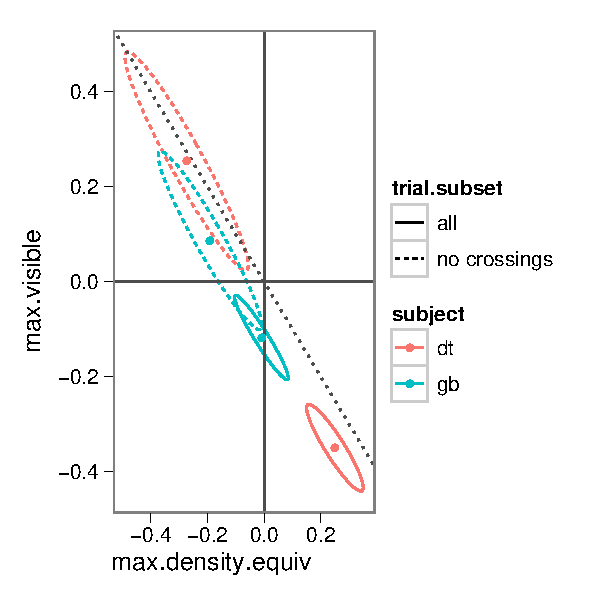
\includegraphics[width=\linewidth]{ellipses_divided}
		\subcaption{Confidence ellipse of the coefficients resulting from logistic regression analysis for each subject. The horizontal axis shows the coefficient $\beta_d$ for target density while the vertical shows the coefficient of $\beta_n$ for target number The graph is scaled to equalize the importance of each variable. Solid ellipses show the results for when all occluded trials are considered; dashed ellipses consider only trials where an element did not cross the boundary of the occluder. }
		\label{fig:densityVersusNumber}
	\end{subfigure}
\begin{subfigure}[b]{.45\linewidth}
	        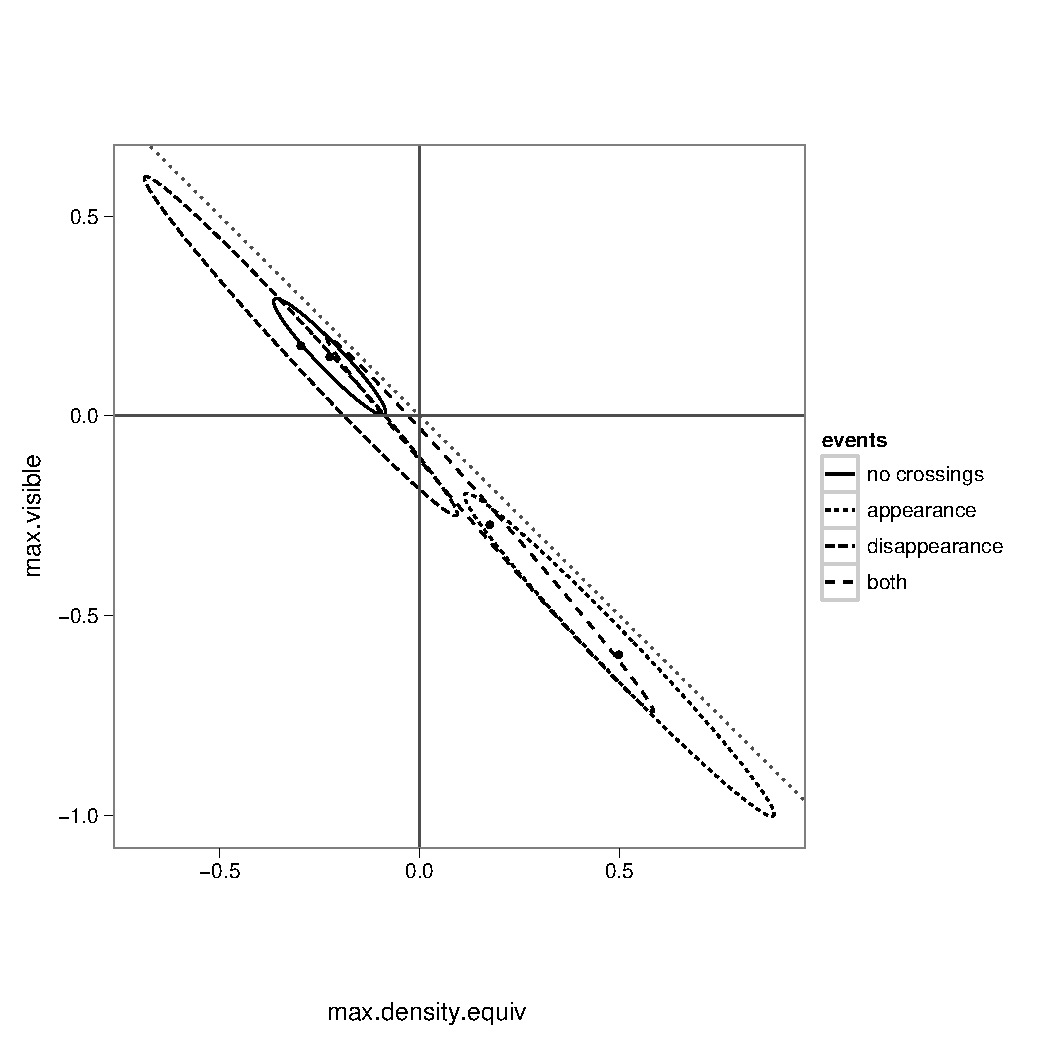
\includegraphics[width=\linewidth]{no_subject}
		\subcaption{With subject data pooled, confidence ellipses for the different trial groups according to whether trials contained appearances or disappearances.  }
		\label{fig:densitySubjectPooled}
	\end{subfigure}
	\caption{Disentangling target number from target density by partially occluding the stimulus.}\label{fig:occlusion}
\end{figure}

The measured PSEs are shown in \autoref{fig:occlusionPSE}. The online estimates from QUEST are disregarded and the PSEs are calculated by fitting a logistic response function with slope, guess and lapse rates varying per subject, as in \autoref{sec:constant}.

If the perceived motion direction were driven by element number rather than element spacing, we might first expect the measured critical spacing to decrease when most targets are occluded. For Subject DT the smallest spacing at PSE were observed in the session where the unoccluded window was in the left hemifeld. In the left hemifield spacing at PSE did not reliably differ between occluded and unoccluded conditions (parametric bootstrap, \ensuremath{p = .16}) In the right hemifield, the spacing at PSE increased for the occluded conditions (\ensuremath{p = .001}). [Author PBM did not show a significant difference in critical spacing between occluded and unoccluded stimuli \todo{this is apparently the case for most data but I need to re-run using the final set of stimulus parameters}]


On the other hand, GB showed a significant decrease in critical spacing for occluded stimuli shown on both sides of the screen (\ensuremath{p < .001}, left; \ensuremath{p < .001}, right.) Over all eccentricities and both hemifields, the average PSE for occluded conditions was $\ensuremath{76\%} \pm \ensuremath{14\%}$ that of unoccluded conditions. \todo{this standard error includes both the estimation uncertainty and the scatter between different conditions, all in one pool. Is that confusing?} This reduction is considerable, but nonetheless there are more elements visible in one hemifield during unoccluded stimuli at PSE than there are in the occluded condition at PSE. In other words the reduction in PSE is not great enough to be accounted for solely by target number.

Nonetheless, in this first measurement, introducing an occluder has mixed effects on the resulting PSE measurement. This may reflect different strategies taken by each subject, or other differences between subjects. Unpacking the components of the display in the occluded condition may reveal an underlying explanation or the different effects, as well as shedding further light on the question of whether it is target number or spacing that is responsible or the reversed direction of perceived motion at high densities.

\subsection{Is density a better predictor than number?}

\todo[inline]{This section wanted to start with addressing the density vs. number question simply, but after plotting the confidence ellipsoids it seems that the approach isn't helpful after all. All it does is lead to a nonsensical result that you have to dive into appearances and disappearances to untangle.}

It is the case that multiple values of target density can result in the same number of elements being present. Contrariwise, the same target density in two different trials can result in different numbers of targets being visible, depending on the randomly selected initial position of the targets (\autoref{fig:occlusionDensity}). This fact may give us leverage to answer the question of whether it is element density or number that determines the perceived direction of motion, since multiple values of target density have been tested with the same number of visible targets and vice versa.

\todo[inline]{In order to even discuss this simplified first stab at the question I need to explain why use $n_{max}$ versus some other count of visible elements. I don't really see a way around it.}


As expanded on below, because elements in the display move behind an occluder, the number of targets visible can change during the stimulus. So the notion of `number of elements visible' for each trial can have different definitions. We considered several measures of element number: the number of targets visible at the onset of motion stimulus ($n_{\mathrm{on}}$); the number of targets visible at the offset of the stimulus ($n_{\mathrm{off}}$); the maximum number of targets visible at any point during the stimulus ($n_{\mathrm{max}}$); the minimum number of targets visible at any point during the stimulus ($n_{\mathrm{min}}$); and the average number of targets visible integrated over the duration of the stimulus ($n_\mathrm{mean}$). Of these variables, by far the best fit to subjects' responses was obtained using $n_{\mathrm{max}}$; the difference in AIC score from the next best contender was 26. Therefore we use $n_{\mathrm{max}}$ for this and subsequent analyses in this section.

\todo[inline]{Note that if you add appearances and disappearances to the model, all these variables  span the same space, so once there's appearances and disappearances, there's no real distinction between any of these variables other than which ones soak up how much variance from certain appearances and disappearances. So am I shooting myself in the foot here, by picking a ``number" alternative that already has some of the effect of appearances and disappearances built in?}

We reconstructed the positions of the elements for each trial and calculated $n_\mathrm{max}$. Then we regressed subjects' responses against two variables, $n_{\mathrm{max}}$ and the corresponding element density $d_\mathrm{max}$. The equivalent element density was defined as the expected maximum number of elements visible in a trial with a given density, taking the expectation over the randomized starting position of the elements. Therefore, $d_\mathrm{max}$ is purely a function of the spacing between targets, and trial-by-trial differences between $d_\mathrm{max}$ and $n_\mathrm{max}$ are due to the randomized starting position of the elements. Regression coefficients of the two variables should thus be directly comparable.

The estimated values of the two regression coefficients are plotted in \autoref{fig:densityVersusNumber} for each subject, along with standard errors drawn as solid ellipses. As expected, since $n_{max}$ and $d_{max}$ are largely correlated, the ellipses are elongated along an axis with slope $-1$, indicating that the two coefficients trade off against each other. The estimated coefficients lie below the diagonal line with slope $-1$, confirming that either added targets, or added density, tended to produce fewer correct answers. However we do not appear to have a consistent answer as to whether density or number of targets produces a better prediction. For instance, in the case of subject DT, the estimated regression coefficients would have an increased number of targets strongly associated with incorrect answers, while increased density strongly promotes correct answers, a situation which is somewhat nonsensical, unless there is a confounding property of the stimulus that correlates with changes of density and number. \todo{``Additionally the residual deviance is probably larger than expected due to overdispersion, indicating that other factors influencing subject's responses have not been accounted for.'' -- quantify?}, Therefore we turn our attention to other visual cues that are present in the stimulus.

\subsection{Appearances and disappearances as confounding cues}

Introducing an occluder unavoidably introduces ancillary visual cues that can give away the global direction of motion even if crowding obscures the direction of motion of flanked elements.  Appearance and disappearance events may provide one cue. As illustrated in (\autoref{fig:occlusionAppearances}), if elements cross the boundary of the trial window, their appearances or disappearances can provide a significant clue to the direction of global motion, since it is global and not local motion direction that determines where appearances and disappearances happen.

Subjects may also be able to exploit the fact that the elements nearest the boundary of the occluder are only flanked on one side; the effect of crowding is much reduced on targets with only one flanker versus targets with flankers on either side \citep{Bouma:1970ng}, so that even if the elements in the midst of the window cannot be spatially distinguished, the `endpoints' of a moving mass of elements might still be successfully tracked thereby giving away the global motion direction. In this scenario, appearance and disappearance events would be deleterious, as they cause the `endpoints' to shift opposite the direction of global motion.

In \autoref{fig:densityVersusNumber} the dashed ellipses show the results of the regression when only trials that do not contain a boundary crossing (appearance or disappearance) are considered. The ellipses are larger due to the reduced sample size, but the data shows that for both subjects, the reversal of apparent motion direction is more likely to be driven by target density than by number. Moreover, when subjects' behavior is stratified by the presence of boundary crossings in the visual stimulus, the differences between subjects' behavior appears to be more consistent with each other, \todo{R tells me that there is still a difference between subjects on appearances, but not on the other three groups} up to a change in intercept. Therefore data from both subjects are pooled in \autoref{fig:densitySubjectPooled}. We see that in aggregate, the data from trials containing no crossings is more consistent with apparent motion reversal being driven by target density than by target number; when all trials are considered, it is the appearances in particular that disguise this fact. We proceeded to try to account for the effect of appearances and disappearances in the regression model. 

\subsection{The effect of appearances and disappearances}


Of the trials with an occluder reported on in \autoref{fig:occlusionPSE},  \ensuremath{ 21 \%} of trials contained an element appearance, \ensuremath{ 21 \%} of trials contained an element disappearance, \ensuremath{ 10 \%} of trials contained both, and \ensuremath{ 68 \%} contained neither. No trials contained more than one appearance or disappearance event.

\todo{This is where the model exploration used to start, before the business with the ellipses. Move the data in this para up or eliminate it?} We first added the predictor $n_{max}$ which was the the maximum number of targets visible during the stimulus presentation. $n_{max}$ was a significant predictor of subjects' responses (Likelihood ratio test, \ensuremath{p < 10^{-4}}). Furthermore, $n_{max}$ was a significant predector among each subset of trials delineated by subject and occlusion condition; (dtleft, \ensuremath{p < 10^{-4}}; dtright, \ensuremath{p = .013}; gbleft, \ensuremath{p = .0013}; gbright, \ensuremath{p < 10^{-4}}). However adding interaction terms for subject and hemifield did not improve the fit, so we did not block $n_{max}$ by those factors.



We then considered the effect of targets appearing from behind the occluder, adding the regressor $n_{app}$, the number of appearance events during each trial. The coefficient for $n_{app}$ was negative ($\beta_{n_{app}} = -1.5 \pm .21$), indicating that appearances increased the rate at which the subjects answered incorrectly (i.e. in agreement with the local direction of motion.) Furthermore, there was a significant interaction \todo{is this the right phrasing? adding interaction coeficients between subject and appearances significantly improved model fit.} between number of appearances and subject identity (\ensuremath{p = .0019}), indicating that appearance events affected different subjects' responses differently. The effect of appearances was considerable compared to the effect of adding targets to the display; for subject GB, the coefficient associated with $n_{app}$ was $.66 \pm .56$ times the coefficient of $n_{max}$; for subject DT the ratio was $1.5 \pm .63$. In other words shifting the initial target position so that an appearance occurs midway through the trial had more effect than adding two or three targets to the unoccluded portion of the display. Differences in the effect of appearances may be due to differing strategies employed by the subjects, and may help to explain the differing effects of occlusion on the PSE values measured for \autoref{fig:occlusionPSE}.


As for disappearances, these also had an effect, although less strongly than appearances. Interestingly, the pattern of effects for disappearances was nearly the inverse of that for appearances: a disappearance generally increased the likelihood of subjects' answering correctly. \todo{I could reference something from MOT literature, like Scholl and Pylyshyn, in assonance with this.} Moreover, the improvement was significant for subject GB ($B_{dis,GB} = .2 \pm .28$, \ensuremath{p = .48}) but did not reach significance for subject DT ($B_{dis,GB} = -0.32 \pm .35$, p = \ensuremath{p = .35}) Overall, including disappearances significantly improved the model fit (\ensuremath{p = .0098}) and the fit was not further improved by stratifying by  subject (\ensuremath{p = .22})\todo{There's a "significant" interaction with GB, left/right side and disappearances; but it's silly to get that specific esp. to get that specific for one subject and not another}.

\todo[inline]{I start to think that the small number of trials with both an appearance and a disappearance are so wacky that they throw a lot of fits off, and we might benefit from leaving them out altogether. But what's a good way to quantify that?

Another thing to think about: I described how appearances could plausibly have either direction of effect (inference of global direction vs. movement of the endpoints.) If in fact both effects are present, that may complicate things and a symptom would be excessive residual deviance in the appearance trials.}

\begin{figure}
	\begin{subfigure}[b]{.45\linewidth}
	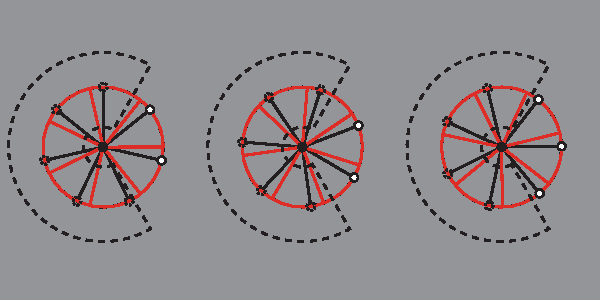
\includegraphics[width=\linewidth]{occlusions}	
	\subcaption{Appearances and disappearances provide additional cues for the direction of motion. The initial position of the targets is shown and the path of their travel is shown as red arrows. Left: a target appears from behind the occluder while the stimulus is visible. Middle: neither an appearance or disappearance occurs during the limited duration of the stimulus. Right: a target disappears behind the occluder while the stimulus is visible. The target density is the same for all three stimuli.}\label{fig:occlusionAppearances}
	\end{subfigure}
	\begin{subfigure}[b]{.45\linewidth}
		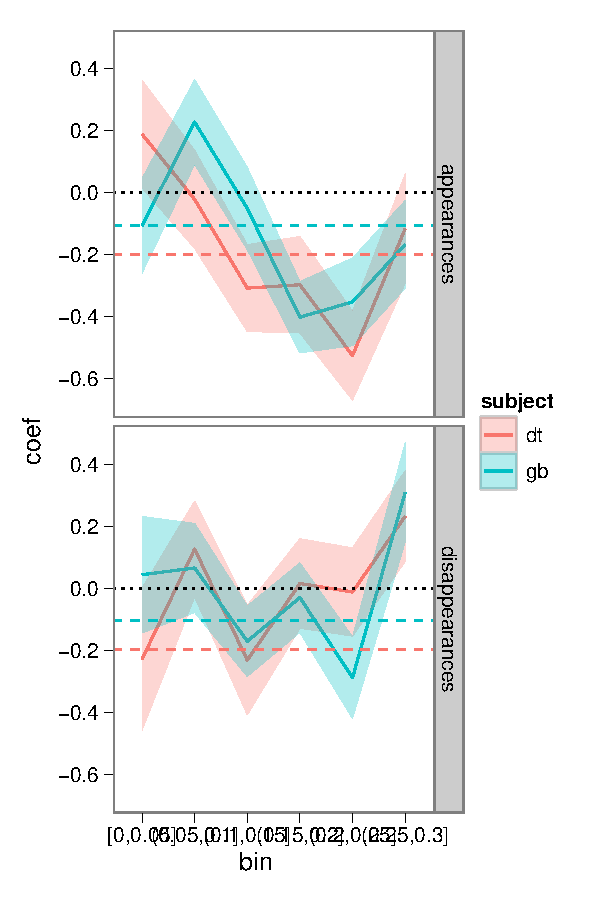
\includegraphics[width=\linewidth]{appearance_timing}
		\subcaption{The effect of appearances on subjects' response rate as a function of time. The horizontal axis divides the stimulus duration into bins. The vertical axis plots the change, in log odds of subjects' rate of answering according to global motion direction, as compared to stimuli that do not contain an appearance or disappearance. Bars indicate standard error of the estimated effect.}\label{fig:appearanceTiming}
	\end{subfigure}
	\caption{Effect of appearance and disappearance events in partially occluded stimuli.}\label{fig:appearances}
\end{figure}

Since appearances have such a marked effect on subjects' responses, we next looked at the timing of appearances within each stimulus presentation. Appearances that occur immediately following stimulus onset or immediately preceding stimulus offset ought not to have much effect on subjects' responses, since the visual stimulus is virtually identical to one that contains no appearance events. On the other hand, appearances that occur during the middle of the stimulus presentation should have a greater effect. To examine the effect of occlusion events as a function of time we stratified the appearance times into equally sized bins. The effect of appearances and disappearances as a function of time is shown in \autoref{fig:appearanceTiming}; for both subjects, the effect of appearances starts near zero and grows significantly negative (associated with responses in the direction of local motion) in the second half of the stimulus presentation. In contrast, the effect of disappearances is smaller, not significantly deviating from zero in these time bins except possibly at the end of the trial.

\todo[inline]{finally, adding density to the equation; show that it obliterates the need for $n_{max}$.}

\todo[inline]{I got stuck on how-to-get-to-this-figure for a bit, since . But then I discovered that a stepwise regression starting with a kitchen-sink of the various factors ends up spitting out a model that drops target-number and keeps target-density as the most significant explanatory variable. Stepwise regression doesn't know anything about the problem domain and proceeds dumbly by significance value ignoring effect size, so I'd like to not use it and have a more traditional discussion, but since a dumb algorithm gets to the right place, that lets me synthesize the key figure.}

\begin{figure}
	\centering
	\begin{subfigure}[b]{.30\linewidth}
	        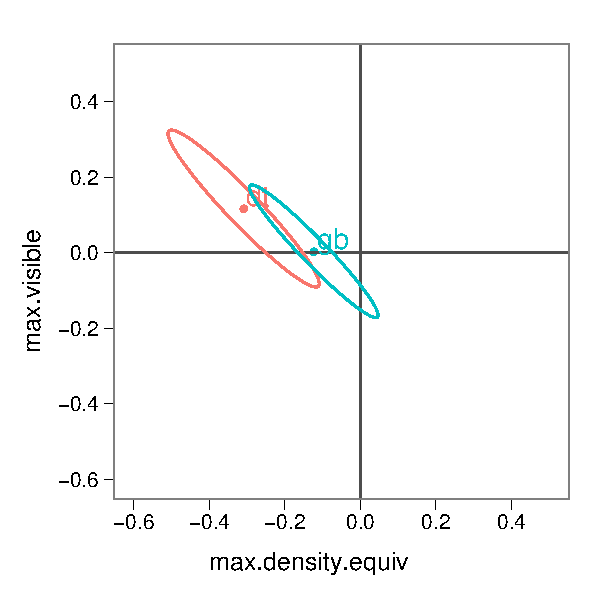
\includegraphics[width=\linewidth]{final_ellipses}
		\subcaption{Confidence ellipses as in \autoref{fig:densityVersusNumber} for the occlusion model, showing the values of both $\beta_d$ for target density while the vertical shows the coefficient of $\beta_n$ for target number. Both subjects' fits are more consistent with target density than with target number.}
		\label{fig:finalEllipses}
	\end{subfigure}
	\begin{subfigure}[b]{.60\linewidth}
		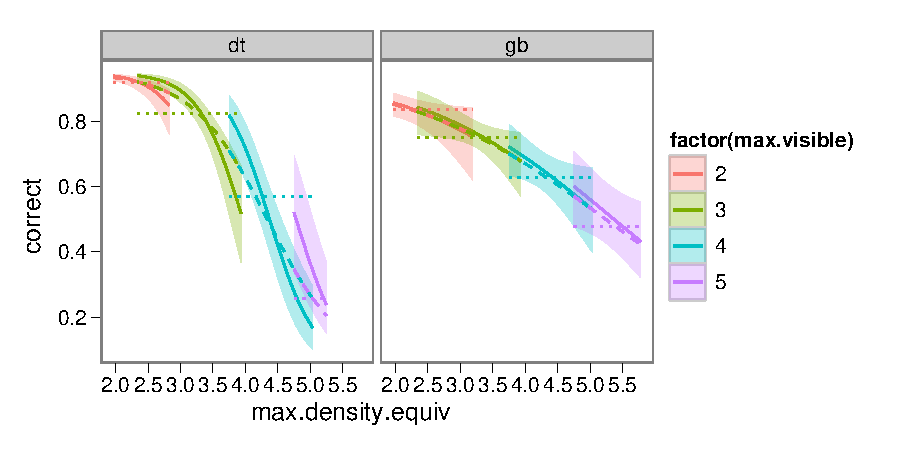
\includegraphics[width=\linewidth]{fancyFigure}	
		\subcaption{Relation between target spacing, target number and subjects' responses. Here data for DT in the left hemifield, and GB in the right hemifield, is used to generate model fits. Each connected line segment represents varying target spacing while holding the number of targets visible in the window. Different colors correspond to different numbers of targets visible in the window, while the equivalent target spacing is plotted along the horizontal axis. Dotted lines indicate predictions made using only element number, and dashed lines show a fit that uses only target spacing. Solid lines and shaded confidence regions are fit allowing a mixture of density and number. The mixture models' results are more compatible with those of the target spacing than those of target number.}\label{fig:occlusionFuncs}
	\end{subfigure}
	\caption{}\label{fig:occlusionModeling}
\end{figure}

Overall, then, in our model which attempts to account for the side effects of occlusion, it appears that element density explains the apparent reversal of motion direction better than element number. We visualize this in two ways. One is to replot the ellipsoids of \autoref{fig:densityVersusNumber}; in \autoref{fig:finalEllipses}, these ellipsoids now draw on data from all occluder trials and account for occlusion side effects, and are more consistent with a main effect of target density than one of number (graphically speaking they place more density on the x-axis than on the y-axis). Another is to draw the predicted psychometric functions resulting from the model, showing how these functions vary in terms of both target number and target density, and what the uncertainty in the prediction is. We do this in \autoref{fig:occlusionFuncs}. Here we compare model fits obtained under three conditions: one in which the subjects' response depends on number (dotted lines), and a model allowing a mixture of the mixture. The same set of interaction variables are used in all fits. In \autoref{fig:occlusionModeling} we only show the data from each subject's better hemifield (left for DT, right for GB.) We observe in that in \autoref{fig:finalEllipses}, for both subjects, the measured coefficients are more consistent with the illusion being driven by element density rather than number. In \autoref{fig:occlusionFuncs} we see that when allowing a mixture of number and density to be used in fitting the psychometric function, the result (solid lines) follows more closely a function based only on density density (dashed lines) than one based only on element number (dotted lines). Thus we assert that the apparent reversal of motion direction is driven by element density.

\todo[inline]{and as a conclusion, now I really ought to update \autoref{fig:occlusionPSE} for the more detailed model.}
\biblio

\end{document}
